\chapter{SO SÁNH TỔNG HỢP VÀ ĐÁNH GIÁ}

\section{Bảng so sánh toàn bộ}

\begin{longtable}{lccccccc}
\caption{Tổng quan tất cả phiên bản YOLO} \\
\toprule
\textbf{Version} & \textbf{Năm} & \textbf{mAP (best)} & \textbf{Params} & \textbf{Anchor} & \textbf{NMS} & \textbf{Multi-Task} & \textbf{Paper} \\
\midrule
\endfirsthead
\toprule
\textbf{Version} & \textbf{Năm} & \textbf{mAP} & \textbf{Params} & \textbf{Anchor} & \textbf{NMS} & \textbf{Multi-Task} & \textbf{Paper} \\
\midrule
\endhead
v1 & 2015 & 63.4\%* & $\sim$45M & Không & Cần & Không & Có \\
v2 & 2016 & 78.6\%* & $\sim$50M & Có & Cần & Không & Có \\
v3 & 2018 & 33.0\% & $\sim$62M & Có & Cần & Không & Có \\
v4 & 2020 & 43.5\% & $\sim$64M & Có & Cần & Không & Có \\
v5 & 2020 & 50.7\% & 86.7M & Có & Cần & Hạn chế & Không \\
v6 & 2022 & 52.5\% & $\sim$58M & Không & Cần & Không & Có \\
v7 & 2022 & 56.8\% & $\sim$71M & Có & Cần & Hạn chế & Có \\
v8 & 2023 & 53.9\% & 68.2M & Không & Cần & 6 tác vụ & Không \\
v9 & 2024 & 55.6\% & 58.1M & Không & Cần & Hạn chế & Có \\
v10 & 2024 & 54.4\% & 29.5M & Không & Không & Không & Có \\
YOLO11 & 2024 & 54.7\% & 56.9M & Không & Không & 6 tác vụ & Không \\
v12 & 2025 & 55.2\% & 59.1M & Không & Không & Có & Có \\
YOLOE & 2025 & 27.1\%** & $\sim$25M & Không & Tùy & Có & Có \\
YOLO26 & 2026 & $\sim$57.2\% & $\sim$60M & Không & Không & 5 tác vụ & Không \\
\bottomrule
\multicolumn{8}{l}{\small *VOC mAP50, **LVIS zero-shot} \\
\end{longtable}

\section{Tiến hóa kiến trúc}

\subsection{Backbone}
\begin{center}
24-layer CNN $\rightarrow$ Darknet-19 $\rightarrow$ Darknet-53 $\rightarrow$ CSPDarknet $\rightarrow$ EfficientRep $\rightarrow$ E-ELAN $\rightarrow$ GELAN $\rightarrow$ Area Attention
\end{center}
\textbf{Xu hướng:} CNN $\rightarrow$ CNN+Residual $\rightarrow$ CSP $\rightarrow$ Re-param $\rightarrow$ Attention-centric

\subsection{Anchor \& NMS}
\begin{center}
Grid (v1) $\rightarrow$ Anchor-based (v2--v7) $\rightarrow$ Anchor-free (v6,v8+) $\rightarrow$ NMS-free (v10+)
\end{center}

\subsection{Loss Function}
\begin{center}
MSE (v1) $\rightarrow$ IoU $\rightarrow$ GIoU $\rightarrow$ CIoU (v4) $\rightarrow$ CIoU+DFL (v8) $\rightarrow$ Bỏ DFL (YOLO26)
\end{center}

\subsection{Framework}
\begin{center}
Darknet C (v1--v4) $\rightarrow$ PyTorch pip install (v5+) $\rightarrow$ Unified API (v8+)
\end{center}

\section{Các phiên bản ``thua'' đời trước}

\begin{table}[H]\centering
\caption{Version thua đời trước — phân tích trade-off}
\begin{tabular}{llll}\toprule
\textbf{Trường hợp} & \textbf{Thua ở đâu} & \textbf{Thắng ở đâu}\\\midrule
v8 thua v7 & mAP: 53.9\% < 56.8\% & Multi-task, ecosystem, dễ dùng \\
v10 thua v9 & mAP: 54.4\% < 55.6\% & Params 2× ít hơn, NMS-free \\
v3 chậm hơn v2 & FPS: 20--51 < 40--67 & Accuracy tốt hơn nhiều \\
\bottomrule
\end{tabular}
\end{table}

\textbf{Nhận xét:} Không version nào thua hoàn toàn. Mỗi ``thua'' là trade-off có chủ đích.

\section{Xếp hạng theo tiêu chí}

\subsection{Accuracy thuần túy (mAP50-95 COCO)}
\begin{enumerate}
    \item YOLO26: $\sim$57.2\%
    \item YOLOv7-E6E: 56.8\%
    \item YOLOv9-E: 55.6\%
    \item YOLOv12-X: 55.2\%
    \item YOLO11-X: 54.7\%
\end{enumerate}

\subsection{Efficiency (mAP/Params)}
YOLOv10-X dẫn đầu: 54.4\% mAP với chỉ 29.5M params (1.84 mAP/M).

\subsection{Đóng góp lý thuyết}
\begin{enumerate}
    \item YOLOv1: Single-stage detection — thay đổi cả lĩnh vực
    \item YOLOv9: Information Bottleneck + PGI — lý thuyết sâu nhất
    \item YOLOv4: BoF/BoS methodology — hệ thống hóa
    \item YOLOv10: NMS-free — giải quyết vấn đề 9 năm
    \item YOLOv12: Attention-centric — mở kỷ nguyên mới
\end{enumerate}

\subsection{Production readiness (2026)}
YOLO11 > YOLOv8 > YOLO26 > YOLOv12

\section{Sơ đồ phả hệ YOLO (Family Tree)}

\begin{figure}[H]
\centering
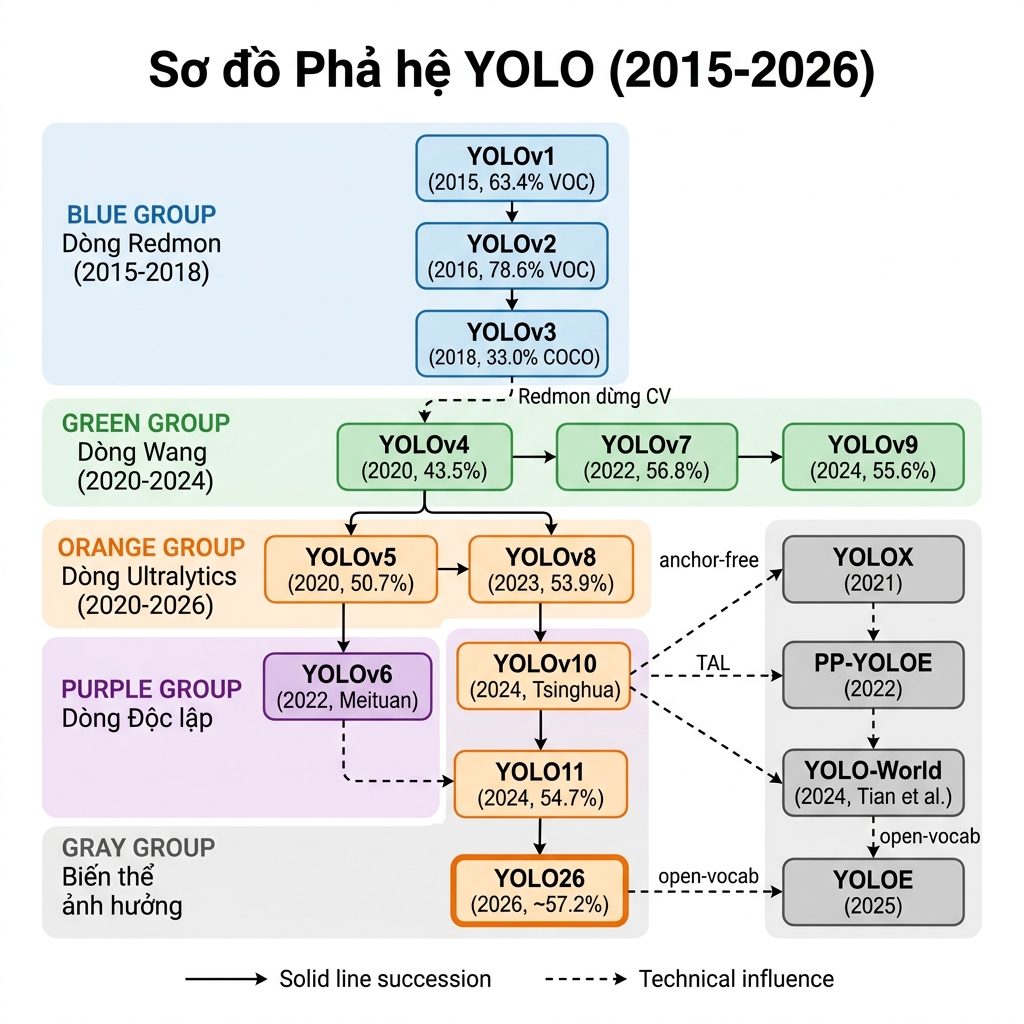
\includegraphics[width=\textwidth]{yolo_family_tree.png}
\caption{Sơ đồ phả hệ các phiên bản YOLO (2015--2026). Đường liền: kế thừa trực tiếp. Đường nét đứt: ảnh hưởng kỹ thuật. Mã nguồn sơ đồ: Mermaid.js (xem file \texttt{yolo\_family\_tree.html}).}
\end{figure}

\section{Xu hướng phát triển}

\begin{enumerate}
    \item \textbf{CNN → Attention:} v12 mở đầu, tương lai sẽ hybrid CNN+Attention
    \item \textbf{Closed-set → Open-vocabulary:} YOLOE cho phép detect vật chưa train
    \item \textbf{Server → Edge:} YOLO26 tối ưu CPU, INT8, mobile
    \item \textbf{NMS → NMS-free:} End-to-end detection từ v10
    \item \textbf{CV ← NLP:} Cross-pollination từ LLM (MuSGD, CLIP)
    \item \textbf{Detection → Multi-task:} 1 model cho detect+segment+pose+track
\end{enumerate}
